\let\negmedspace\undefined
\let\negthickspace\undefined
\documentclass[journal,12pt,onecolumn]{IEEEtran}
\usepackage{cite}
\usepackage{amsmath,amssymb,amsfonts,amsthm}
\usepackage{algorithmic}
\usepackage{graphicx}
\graphicspath{{./figs/}}
\usepackage{textcomp}
\usepackage{xcolor}
\usepackage{txfonts}
\usepackage{listings}
\usepackage{enumitem}
\usepackage{mathtools}
\usepackage{gensymb}
\usepackage{comment}
\usepackage{caption}
\usepackage[breaklinks=true]{hyperref}
\usepackage{tkz-euclide} 
\usepackage{listings}
\usepackage{gvv}                                        
%\def\inputGnumericTable{}                                 
\usepackage[latin1]{inputenc}     
\usepackage{xparse}
\usepackage{color}                                            
\usepackage{array}
\usepackage{longtable}                                       
\usepackage{calc}                                             
\usepackage{multirow}
\usepackage{multicol}
\usepackage{hhline}                                           
\usepackage{ifthen}                                           
\usepackage{lscape}
\usepackage{tabularx}
\usepackage{array}
\usepackage{float}
\newtheorem{theorem}{Theorem}[section]
\newtheorem{problem}{Problem}
\newtheorem{proposition}{Proposition}[section]
\newtheorem{lemma}{Lemma}[section]
\newtheorem{corollary}[theorem]{Corollary}
\newtheorem{example}{Example}[section]
\newtheorem{definition}[problem]{Definition}
\newcommand{\BEQA}{\begin{eqnarray}}
\newcommand{\EEQA}{\end{eqnarray}}
\newcommand{\define}{\stackrel{\triangle}{=}}
\theoremstyle{remark}
\newtheorem{rem}{Remark}

\begin{document}

\title{8.2.23}
\author{ee25btech11056 - Suraj.N}
\maketitle
\renewcommand{\thefigure}{\theenumi}
\renewcommand{\thetable}{\theenumi}

\begin{document}

\textbf{Question :} The conic has vertices $\,(0,\pm 13)\,$ and foci $\,(0,\pm 5)\,$. Find the equation of the conic.

\textbf{Solution :} 

\begin{table}[h!]
  \centering
  \begin{tabular}{|c|c|}
\hline
\textbf{Name} & \textbf{Value} \\ \hline
$\vec{A}$ & $\myvec{2 & 1 \\0 & 3}$ \\ \hline
\end{tabular}

  \caption*{Table : Ellipse}
  \label{8.2.23}
\end{table}

The conic has two foci , so it cannot be a parabola .

Equation for any conic with directrix $\vec{n}^\top\vec{x} = c$ , eccentricity e and focus $\vec{F}$ is given by 

\begin{align}
  \vec{x}^\top\vec{V}\vec{x} + 2\vec{u}^\top\vec{x} + f &= 0 \label{eq:conic} \\
\end{align}

\begin{align}
  \vec{V} &= \norm{\vec{n}}^2\vec{I} - e^2\vec{n}\vec{n}^\top \label{eq:matrixV} \\
  \vec{u} &= ce^2\vec{n} - \norm{\vec{n}}^2\vec{F} \label{eq:matrixu} \\
  f &= \norm{\vec{n}}^2\norm{\vec{F}}^2 - c^2e^2 \label{eq:f}
\end{align}

The normal vector of the directrix is along the direction vector of $\vec{F_1} - \vec{F_2}$

\begin{align}
  \vec{n} &= \vec{F_1} - \vec{F_2} \equiv \vec{e_2}
\end{align}

From \eqref{eq:matrixV} we can form the matrix $\vec{V}$

\begin{align}
  \vec{V} &= \myvec{1 & 0\\0 & 1} - e^2\myvec{0 & 0\\0 & 1}\\
  \vec{V} &= \myvec{1 & 0\\0 & 1 - e^2}
\end{align}

As $\vec{V}$ is an upper triangular matrix , we get the eigen values as the diagonal entries 

\begin{align}
  \lambda_1 &= 1 - e^2 & \lambda_2 = 1
\end{align}

Clearly $\mydet{\vec{V}} \neq 0$ , $\vec{V}^{-1}$ exists.

\pagebreak

The center of the conic $\vec{c}$ can be found 

\begin{align}
  \vec{c} &= \frac{\vec{F_1}+\vec{F_2}}{2} = \vec{0}
\end{align}

The relation between the $\vec{c}$ , $\vec{V}$ and $\vec{u}$ is given by 

\begin{align}
  \vec{V}\vec{c} + \vec{u} &= \vec{0} & \mydet{\vec{V}} \neq 0 \\
  \vec{c} &= \vec{0}\\
  \vec{u} &= \vec{0}
\end{align}

From \eqref{eq:matrixu} we get 

\begin{align}
  ce^2\vec{e_2} &= \vec{F_1}\\
  \myvec{0\\ce^2} &= \myvec{0\\5}\\
  ce^2 &= 5\\
  c &= \frac{5}{e^2} \label{eq:c}
\end{align}

\begin{align}
  f_0 &= \vec{u}^\top\vec{V}^{-1}\vec{u} - f
\end{align}

as $\vec{u}=\vec{0}$ and from \eqref{eq:f}, we get 

\begin{align}
  f_0 &= c^2e^2 - 25 
\end{align}

The length of the major axis is the distance between the two vertices 

\begin{align}
  \norm{\vec{B_1}-\vec{B_2}} &= 26
\end{align}

The length of major axes is also given as 

\begin{align}
  2\sqrt{\left|\frac{f_0}{\lambda_1}\right|}
\end{align}

So,

\begin{align}
  2\sqrt{\left|\frac{c^2e^2 - 25}{1 - e^2}\right|} &= 26
\end{align}

From \eqref{eq:c} we get 

\begin{align}
  \sqrt{\frac{25}{e^2}} &= 13\\
  \frac{5}{e} &= 13\\
  e &= \frac{5}{13}
\end{align}

\pagebreak

As e \textless 1 , the conic is an \textbf{ellipse}

The value of c and directix equation are given as 

\begin{align}
  c &= \frac{169}{5} & \vec{n}^\top\vec{x} = \pm \frac{169}{5}
\end{align}

Using the obtained values of c and e , we get 

\begin{align}
  \vec{V} &= \myvec{1 & 0\\0 & \tfrac{144}{169}}\\
  \vec{u} &= \vec{0}\\
  f &= -144
\end{align}

Substituting these in \eqref{eq:conic} , we get the equation of \textbf{ellipse} as 

\begin{align}
  \vec{x}^\top\myvec{\tfrac{1}{144} & 0\\0 & \tfrac{1}{169}}\vec{x} &= 1\\
\end{align}

\pagebreak

\begin{figure}[h!]
  \centering
  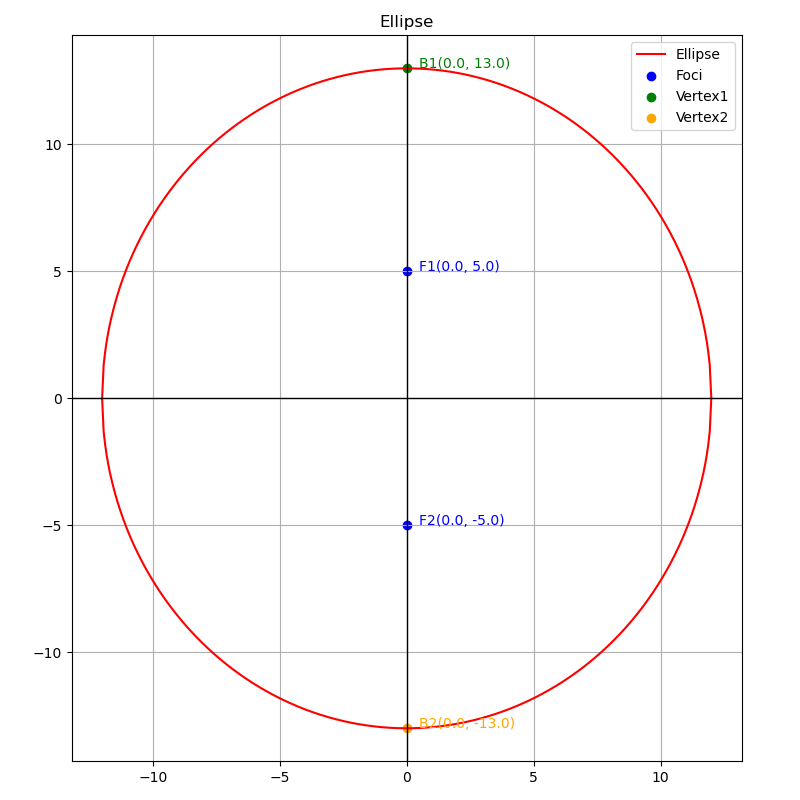
\includegraphics[width=0.7\columnwidth]{figs/ellipse.png} 
   \caption*{Fig : Ellipse}
  \label{Fig1}
\end{figure}



\end{document}
